\chapter{Results}
\label{results}

\section{Phase One Results}
\label{results:userStudyPhaseOne}

In this phase, we recorded \uniqueUsersPhaseOneUserStudy users reciting any of \numOronymsPhaseOneUserStudy oronyms of the phrase ``an ice cold hour", or any of the \numForthRightOohOronymPhrases oronyms for the phrase ``fourth rye to".  Out of \numResponsesPhaseOneUserStudy recordings, only the recordings of the oronyms of ``fourth rye to" were found to diverge from our excepted phonetic patterns, likely due to poor microphone quality not being able to pick up the aspriated \emph{`f'} sound at the beginning of the phrase\cite{elko_electronic_2007}.



\section{Phase Two Results}
\label{results:userStudyPhaseTwo}

Our top five transcribed oronyms, as seen in table ~\ref{table:fullFreqVsActual}, were ``an ice cold hour", ``a nice cold hour", ``a nice gold hour", ``on ice cold hour", and ``in ice cold hour". All of these were predicted by our oronym-generator, except for ``a nice gold hour".  This is a known limitation of MisheardMe Oronym Tree, though, because we chose to focus on exact phonetic matches.  The cold/gold mishearing is a product of phoneme voiced/voiceless pair swapping, which we cover in-depth in section ~\ref{section:phonemeSwapping}. It is outside the current scope of our project. 


\begin{figure}
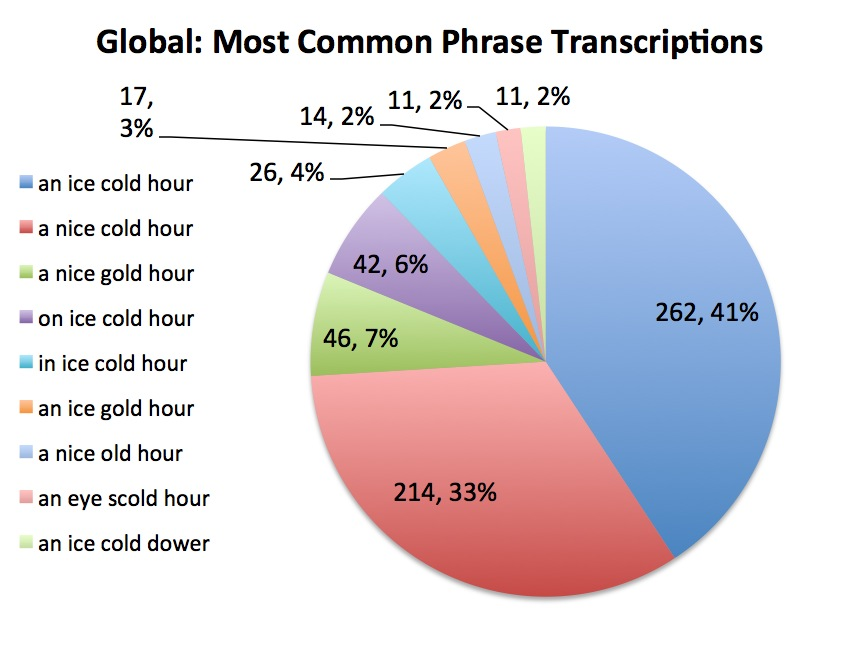
\includegraphics[width=150mm]{mostCommonTranscriptionsPieChartGlobal.jpg}
\captionfonts
\caption[Most Common Transcriptions Globally]{ Our top two transcriptions were ``a nice cold hour" and ``an ice cold hour" }
\label{fig:mostCommonTranscriptionsPieChartGlobal}
\end{figure}


\begin{table}
\begin{center}
\begin{tabular}{ | l | l | l | c | }
\hline 
predicted freq & phrase transcribed & total answers \\
\hline 
931028 &  an ice cold hour &  262 \\
\hline
7851662&   a nice cold hour &  214  \\
\hline
0  & a nice gold hour &  46 \\
\hline
2911102 &  on ice cold hour &  42 \\
\hline
5503158&   in ice cold hour &  26 \\
\hline
0 &  an ice gold hour &  17 \\
\hline
8013781 &  a nice old hour&   14 \\
\hline
892949&   an ice cold dower &  11 \\
\hline
859307 &  an eye scold hour &  11 \\
\hline
\hline 
\end{tabular}
\captionfonts
\caption[Phrase word frequency sum vs times transcribed]{ In this table, we list all oronyms that were transcribed more than five times. Out of this list, all but two the two containing the word ``gold" were predicted by our oronym algorithm.  We expected that any voiced/voiceless phoneme substitutions would be missed by our algorithm. }
\label{table:fullFreqVsActual}
\end{center}
\end{table}


\begin{figure}
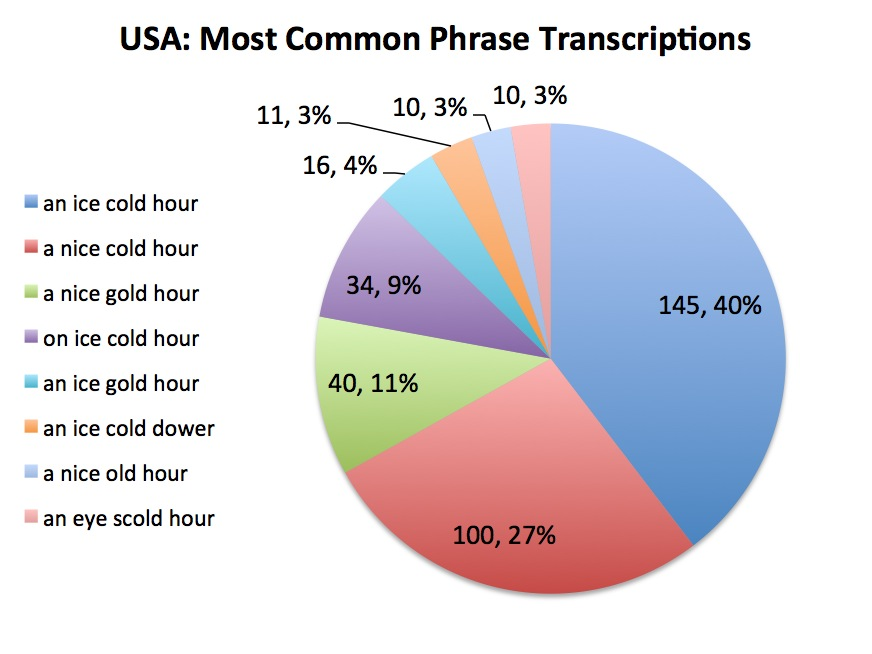
\includegraphics[width=150mm]{mostCommonTranscriptionsPieChartUSA.jpg}
\captionfonts
\caption[Most Common Transcriptions from American respondents]{ Though the breakdown is a bit different than the global transcription breakdown, you can still see the clear trend of ``a nice cold hour" and ``an ice cold hour" being the most common.  There is a slightly larger gap between these two phrase, we hypothesize, because the American transcribers are familiar with what words normally are in proximity to others. }
\label{fig:mostCommonTranscriptionsPieChartUSA}
\end{figure}



\subsection{Transcription oronyms' actual frequency vs calculated frequency}

Though the most commonly transcribed phrases were found by our oronym generation, figure ~\ref{fig:AllTranscriptionsBubbleChart} shows an unexpected distribution of the number of times each phrase was recorded versus the frequency metric that we calculated. We hypothesized that a simple summation of the UNISYN-provided word frequency for each word in a phrase would give a semi-meaningful indicator of whether a phrase's likelyhood to be heard.  

\begin{figure}
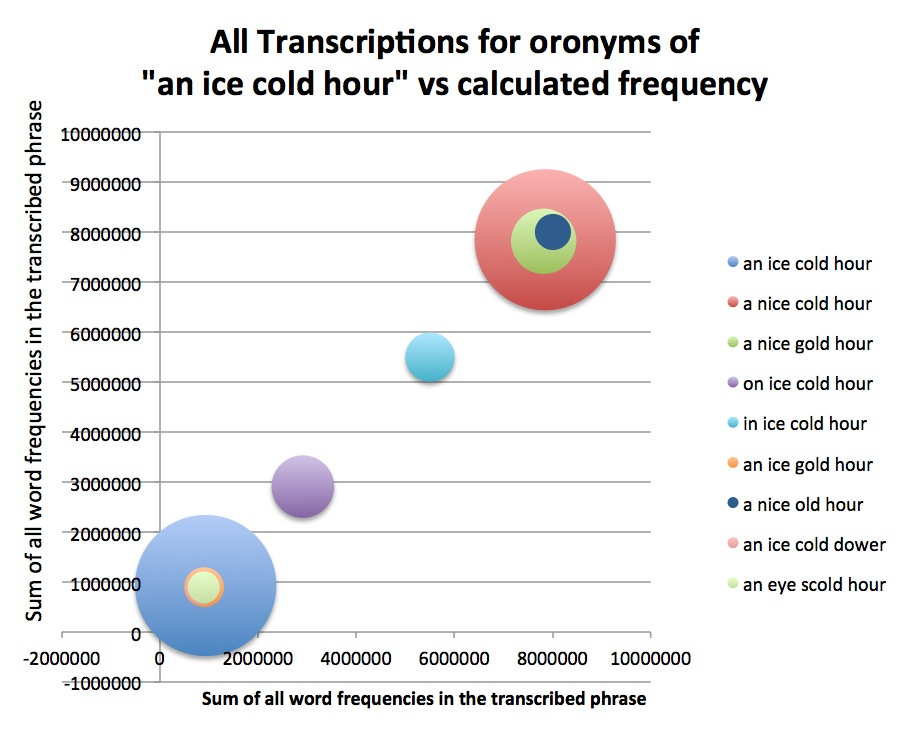
\includegraphics[width=150mm]{AllTranscriptionsBubbleChart.jpg}
\captionfonts
\caption[Bubble Chart of All Transcribed Phrases mapped against their predicted frequency]{Bubble Chart of All Transcribed Phrases mapped against their predicted frequency}
\label{fig:AllTranscriptionsBubbleChart}
\end{figure}


Unfortunately, that proved not to be the case.  In figure ~\ref{fig:blockParseStack_MechTurkAnswers}, we see a 2d block version of our 3d oronym parse tree, as it looks when only considering the transcriptions that were actually entered. If our frequency metric was valid, we would see that figure ~\ref{fig:blockParseStack_predictedMechTurkAnswers} would resemble figure~\ref{fig:blockParseStack_MechTurkAnswers}.  Past the first branch, they only vaguely resember eachother, showing that our frequency metric could use some improvement. 

\begin{figure}
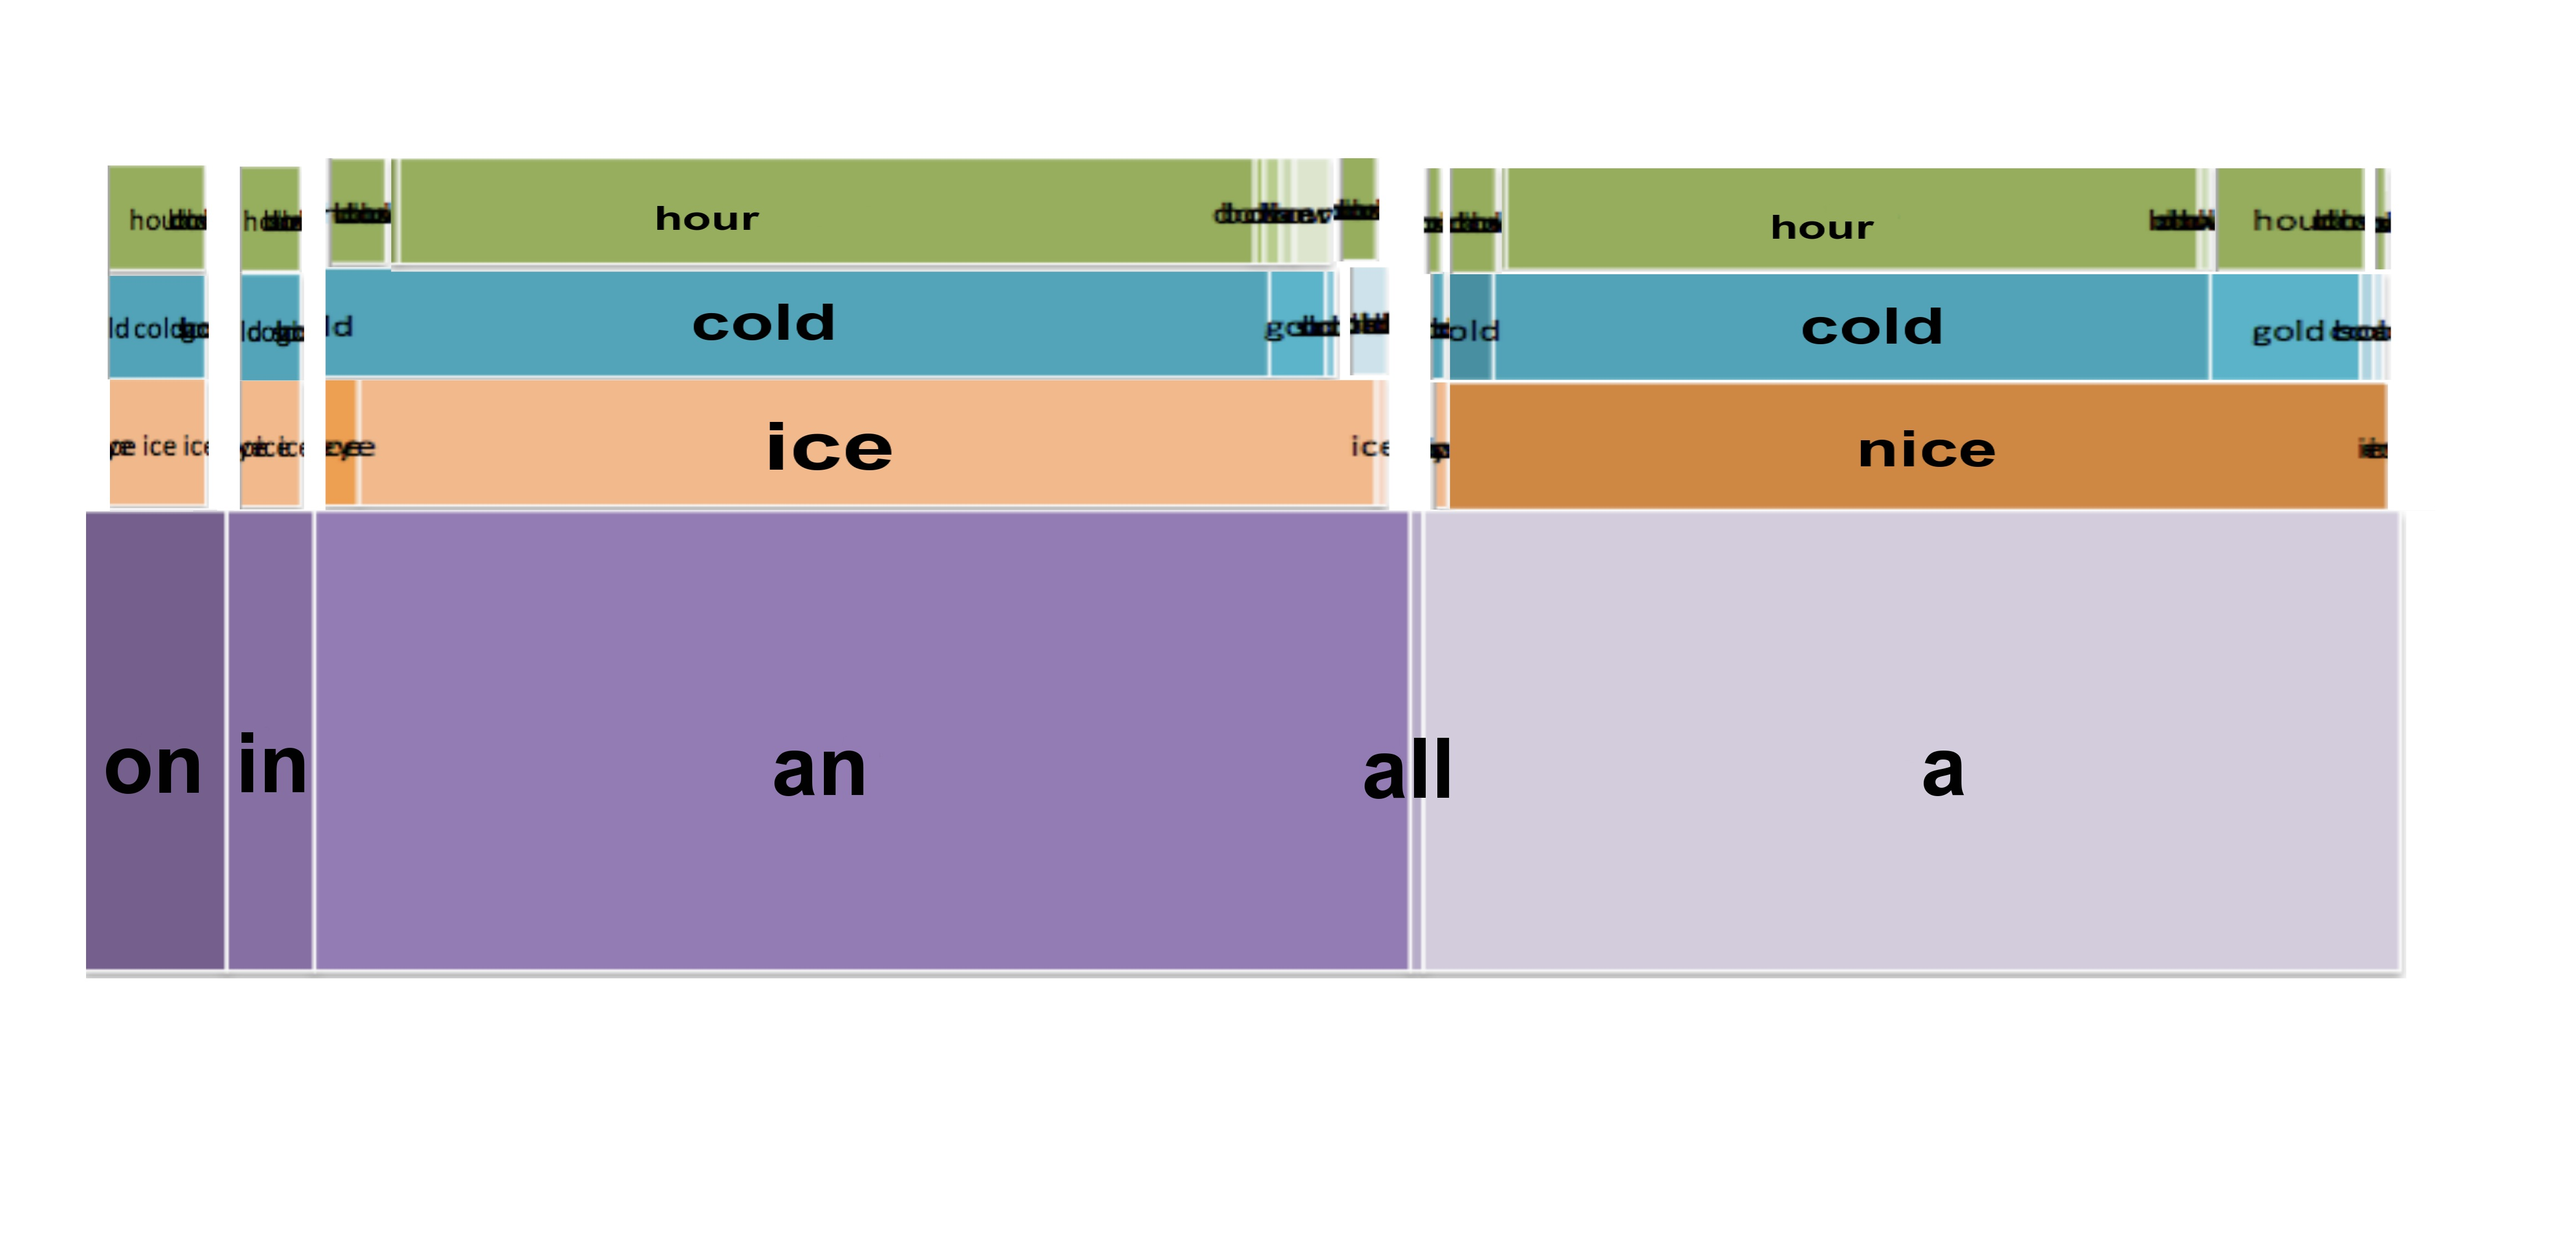
\includegraphics[width=150mm]{mechTurkAnswersAllStackedBars.jpg}
\captionfonts
\caption[2d block version of our 3d oronym parse tree]{2d block version of our 3d oronym parse tree, containing all the transcribed oronyms from mechanical turk. Instead of branches with varying radiuses, we have blocks that are scaled by the number of times that word occurs after the word block it is on top of.}
\label{fig:blockParseStack_MechTurkAnswers}
\end{figure}


\begin{figure}
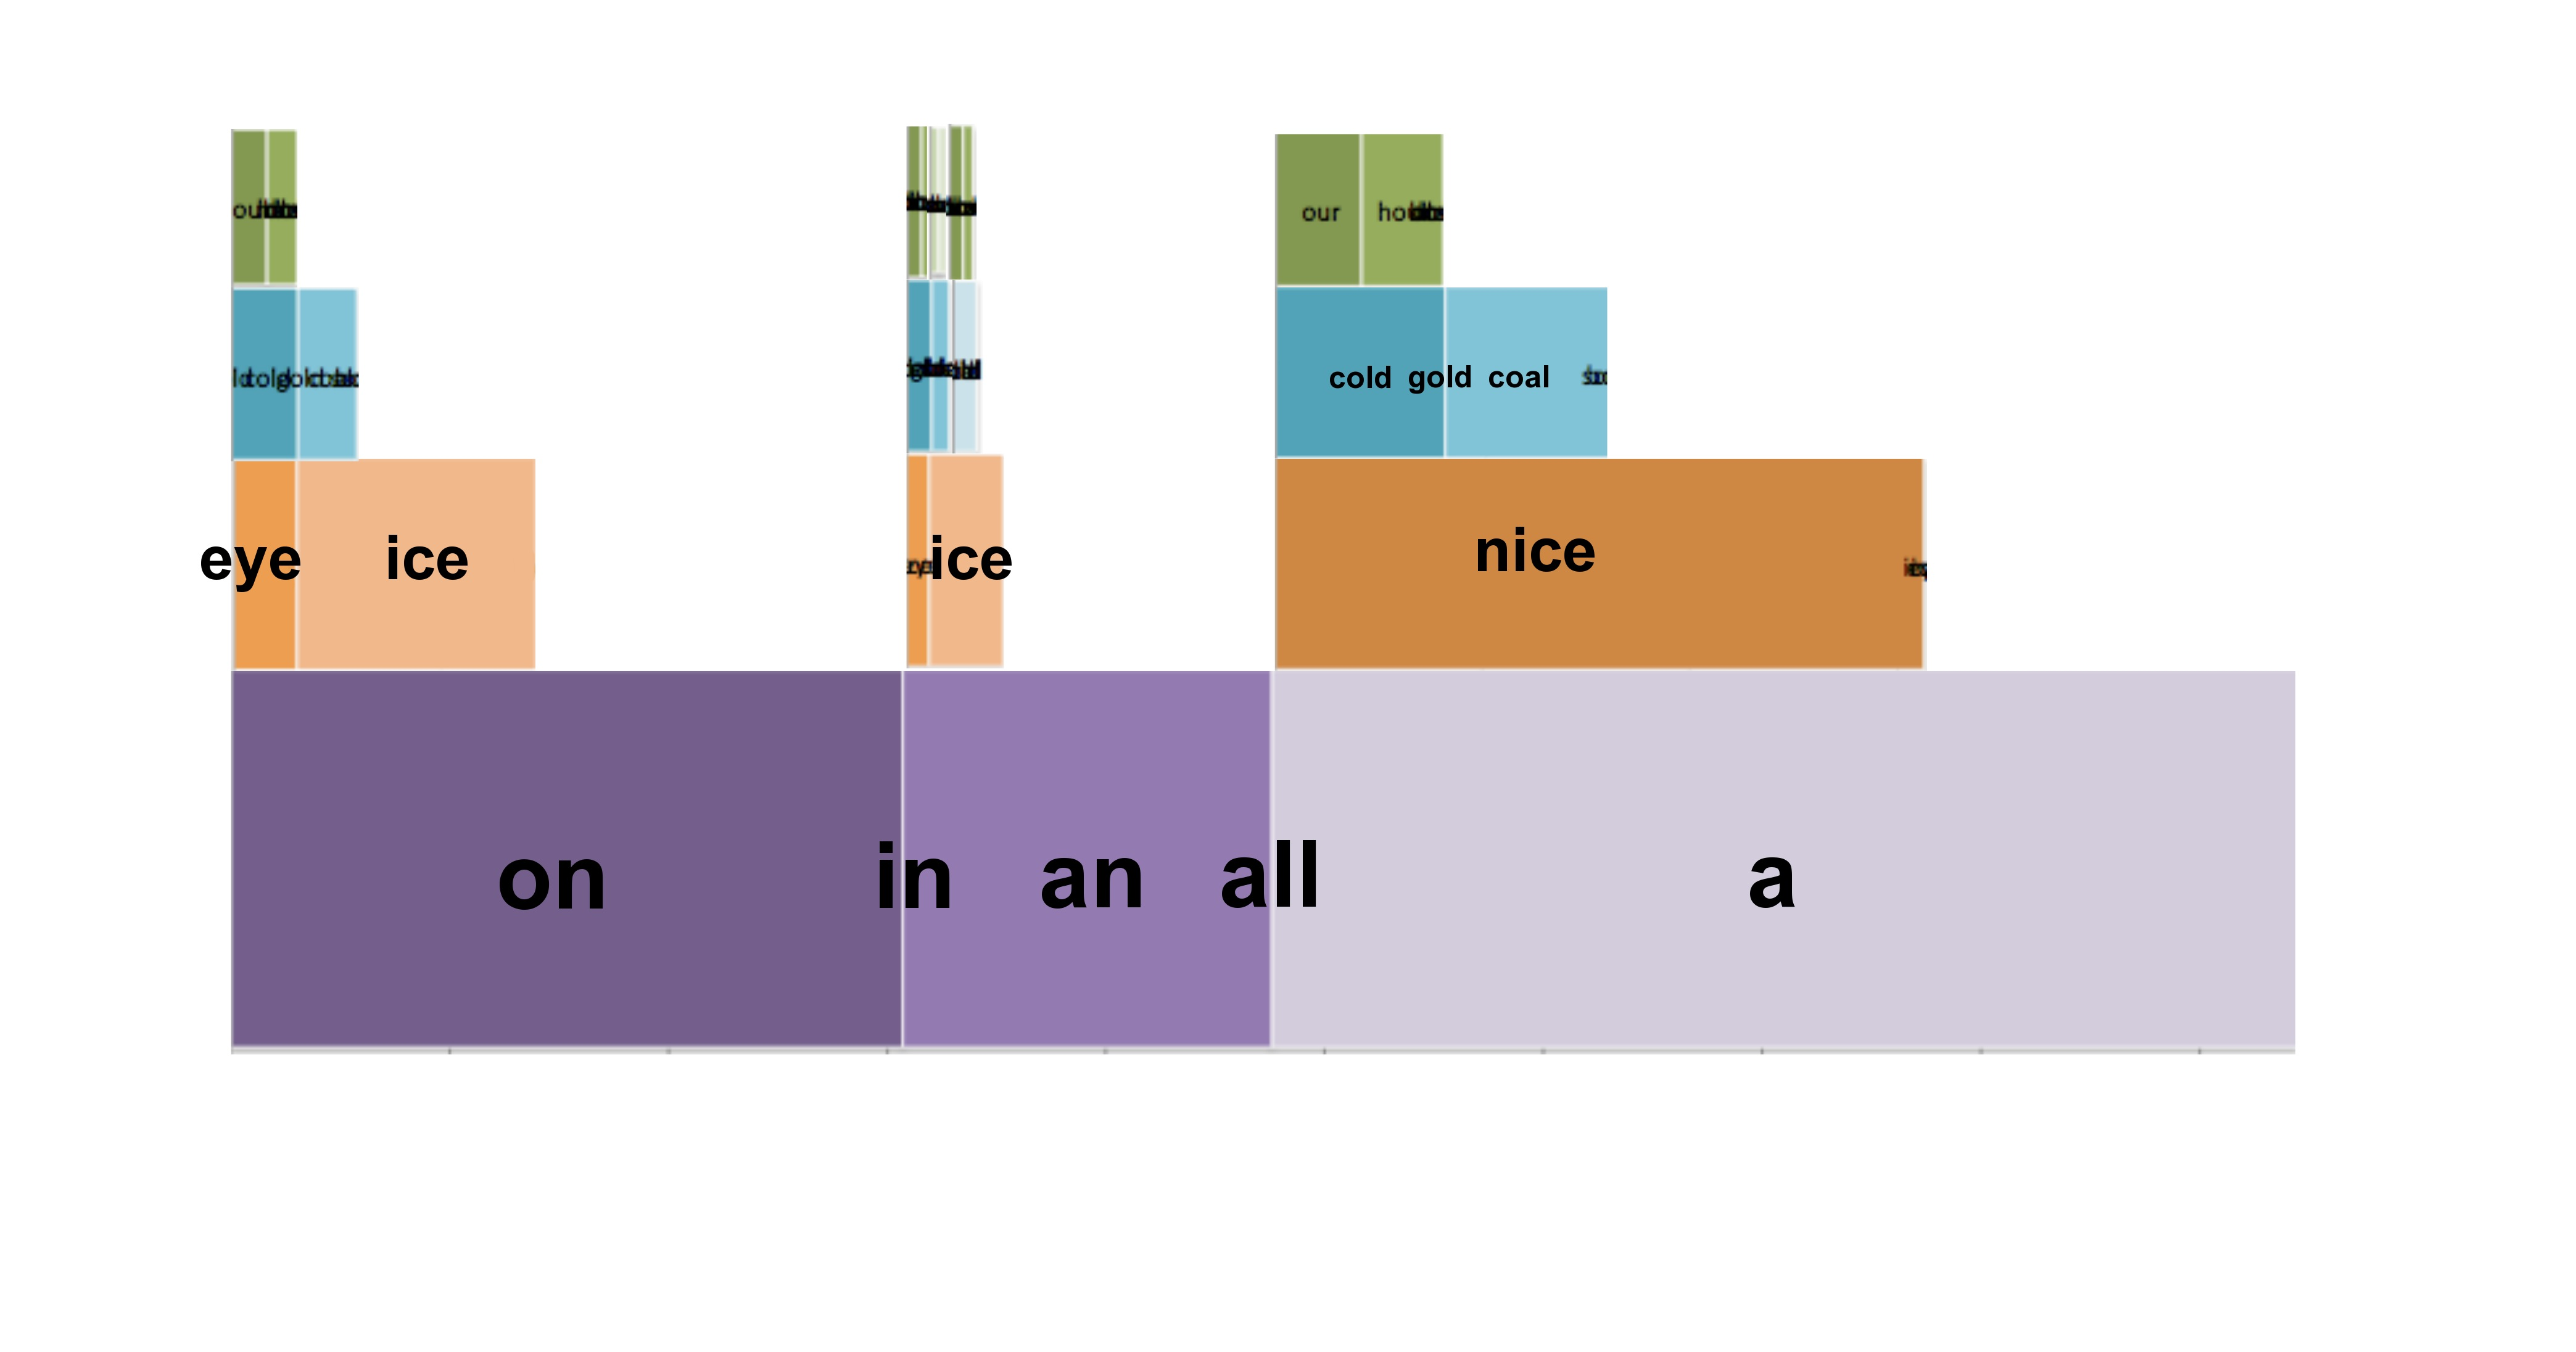
\includegraphics[width=150mm]{mechTurkStackedBars_scaledToPredictedFrequency.jpg}
\captionfonts
\caption[Mechanical Turk Transcriptions in Predictive Freq 2D Block ``Parse Tree"]{If our predictive frequency metric were completely correct, then this would be a solid block. Each filled-in part is a transcription that was actually typed by a person.  All the empty spaces represent oronyms that our frequency metric incorrectly predicted would be likely to be transcribed. }
\label{fig:blockParseStack_predictedMechTurkAnswers}
\end{figure}

